% ------------------------------------------------------------------------
% -*-TeX-*- -*-Hard-*- Smart Wrapping
% ------------------------------------------------------------------------
% AMS-LaTeX definitions:     Thesis ++++ Alex, September 1994 ************
% ------------------------------------------------------------------------
% Ph.D. Thesis Defended on November 25, 1994
% ------------------------------------------------------------------------
\documentclass[12pt]{report}
\usepackage[centertags]{amsmath}
\usepackage{amsfonts}
\usepackage{amssymb}
\usepackage{amsthm}
\usepackage{newlfont}
\usepackage{xthesis} %DAL Thesis Style
\usepackage{xtocinc} %Include Table of Contents as the first entry in TOC
\usepackage{graphicx}
\usepackage[toc,page]{appendix}
\usepackage{makeidx}
\usepackage{fixltx2e}
\usepackage{mathtools}
%                     Faculty of Grad Studies insists on this!?
%\usepackage[active]{srcltx}  %SRC Specials for DVI search
% Fuzz -------------------------------------------------------------------
\hfuzz2pt % Don't bother to report over-full boxes if over-edge is < 2pt
% Line spacing -----------------------------------------------------------
\newlength{\defbaselineskip}
\setlength{\defbaselineskip}{\baselineskip}
\newcommand{\setlinespacing}[1]%
           {\setlength{\baselineskip}{#1 \defbaselineskip}}
\newcommand{\doublespacing}{\setlength{\baselineskip}%
                           {2.0 \defbaselineskip}}
\newcommand{\singlespacing}{\setlength{\baselineskip}{\defbaselineskip}}
% MATH -------------------------------------------------------------------
\newcommand{\A}{{\cal A}}
\newcommand{\h}{{\cal H}}
\newcommand{\s}{{\cal S}}
\newcommand{\W}{{\cal W}}
\newcommand{\BH}{\mathbf B(\cal H)}
\newcommand{\KH}{\cal  K(\cal H)}
\newcommand{\Real}{\mathbb R}
\newcommand{\Complex}{\mathbb C}
\newcommand{\Field}{\mathbb F}
\newcommand{\RPlus}{[0,\infty)}
%
\newcommand{\norm}[1]{\left\Vert#1\right\Vert}
\newcommand{\essnorm}[1]{\norm{#1}_{\text{\rm\normalshape ess}}}
\newcommand{\abs}[1]{\left\vert#1\right\vert}
\newcommand{\set}[1]{\left\{#1\right\}}
\newcommand{\seq}[1]{\left<#1\right>}
\newcommand{\eps}{\varepsilon}
\newcommand{\To}{\longrightarrow}
\newcommand{\RE}{\operatorname{Re}}
\newcommand{\IM}{\operatorname{Im}}
\newcommand{\Poly}{{\cal{P}}(E)}
\newcommand{\EssD}{{\cal{D}}}
% THEOREMS ---------------------------------------------------------------
\theoremstyle{plain}
\newtheorem{thm}{Theorem}[section]
\newtheorem{cor}[thm]{Corollary}
\newtheorem{lem}[thm]{Lemma}
\newtheorem{prop}[thm]{Proposition}
%
\theoremstyle{definition}
\newtheorem{defn}{Definition}[section]
%
\theoremstyle{remark}
\newtheorem{rem}{Remark}[section]
%
\numberwithin{equation}{section}
\renewcommand{\theequation}{\thesection.\arabic{equation}}
%%% ----------------------------------------------------------------------
\setlength{\tclineskip}{1.05\baselineskip}
%%% ----------------------------------------------------------------------
%\nobib
%\draft
%\nofront

\dedicate{To all the people who works for open sources projects out of no personal benefit}
\copyrightyear{2015}
\submitdate{2015}
%\convocation{May}{1995}

% ------------------------------------------------------------------------

\title{Detection of  Fraudulent Activities in Online Communities}

\author{Mostafizur Rahman \& Mujahidul Islam}

\supervisor{Dr. S. M. Farhad}
\university{Bangladesh University Of Engineering And Technology}	
\address{Dhaka 1000}		
\dept{Computer Science And Engineering}
\faculty{Electrical and Electronic Engineering }
\degree{Bachelor Of Science}
\permissionfalse


% ------------------------------------------------------------------------
\makeindex
\begin{document}
{
\typeout{:?000000000} % Don't bother with over/under-full boxes
\beforepreface
\typeout{:?111111111} % Process All Errors from Here on
}
% ------------------------------------------------------------------------
%\setcounter{page}{1}
%\tableofcontents
%\listoffigures
%\listoftables
% ------------------------------------------------------------------------
{
\typeout{Abstract}
\include{ABS}
}
% ------------------------------------------------------------------------
{
\typeout{Acknowledgements}
\include{ACK}
}
% ------------------------------------------------------------------------
\afterpreface
\def\baselinestretch{1}
\setlinespacing{1.66}
% ------------------------------------------------------------------------
{
%\typeout{Introduction}
\chapter{Introduction}
Online communities have become very popular in the recent times. They have become incredibly helpful in sharing knowledge, ideas, skills or even experiences nowadays. People ask questions on different topics and others who have knowledge on that topic reply to those questions. Thus a knowledge sharing culture has already grown and it's getting a proper shape slowly. A number of QA sites and we based discussion forum are being widely used by millions of users across the world. So it's important to make sure that the knowledge base is not corrupted. In this paper we will introduce major fradulant activities which are frequently found in online communities and also propose different approaches to classify those fradulant activities properly. 


\section{Motiovation}
There is no doubt that the online communities are playing a vital role in learning new things and sharing knowledge. But there is no guaranty that the answer someone has given is absolutely correct. There must be strong logic and references to the answer to be a good one. Thus, awarding some points and other rewards like badges, medals and other cool stuffs to the answerer has become a popular mean to encourage to provide more quality answers. This has somewhat established a trend that the more points and other rewards a person has, the more he knows. 
\\
One of the most widely used 


\chapter{Related Works}

This section examines major and commonly used techniques and algorithms.
\section{Overview}
\begin{figure}
  \centering
  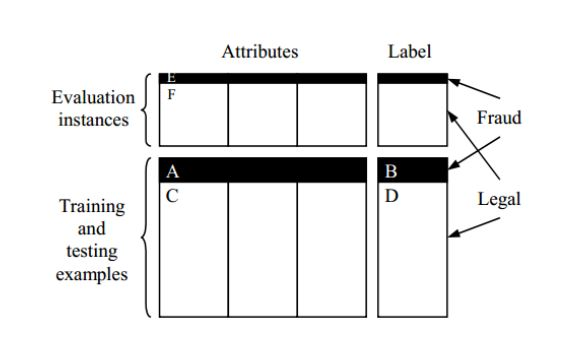
\includegraphics[width=10cm]{related_works}
  \caption{ Structured diagram of the possible data for analysis. Data
mining approaches can utilise training/testing data with labels, only legal
examples, and no labels to predict/describe the evaluation data.}\label{overview_fig}
\end{figure}

Figure \cite{overview_fig} shows that many existing fraud detection systems
typically operate by adding fraudulent claims/applications/
transactions/accounts/sequences (A) to “black lists” to match for likely
frauds in the new instances (E). Some use hard-coded rules which each
transaction should meet such as matching addresses and phone numbers, and
price and amount limits (Sherman, 2002).

Below outlines the complex nature of data used for fraud detection in general
(Fawcett, 2003; 1997):

\begin{itemize}
  \item Volume of both fraud and legal classes will fluctuate independently
      of each other; therefore class distributions (proportion of
      illegitimate examples to legitimate examples) will change over time.
  \item Multiple styles of fraud can happen at around the same time. Each
      style can have a regular, occasional, seasonal, or onceoff temporal
      characteristic.
  \item Legal characteristics/behaviour can change over time.
\end{itemize}

\par
1) Labelled training data (A + B + C + D) can be processed by single
supervised algorithms. A better suggestion is to employ hybrids such as
multiple supervised algorithms , or both supervised and unsupervised
algorithms to output suspicion scores, rules and/or visual anomalies on
evaluation data.
\par
2) All known legal claims/applications/transactions/accounts/ sequences (C)
should be used processed by semi-supervised algorithms to detect significant
anomalies from consistent normal behaviour.
\par
3) Combining training data (the class labels are not required here) with
evaluation data (A + C + E + F). These should be processed by single or
multiple unsupervised algorithms to output suspicion scores, rules and/or
visual anomalies on evaluation data.


\section{Supervised Approaches on Labelled Data (A + B + C + D)}
Predictive supervised algorithms examine all previous labelled transactions
to mathematically determine how a standard fraudulent transaction looks like
by assigning a risk score (Sherman, 2002). Neural networks are popular and
support vector machines (SVMs) have been applied. Ghosh and Reilly (1994)
used a three-layer, feed-forward Radial Basis Function (RBF) neural network
with only two training passes needed to produce a fraud score in every two
hours for new credit card transactions. Barse et al (2003) used a multi-layer
neural network with exponential trace memory to handle temporal dependencies
in synthetic Video-on-Demand log data. Syeda et al (2002) propose fuzzy
neural networks on parallel machines to speed up rule production for
customer-specific credit card fraud detection.

\par
The neural network and Bayesian network comparison study (Maes et al, 2002)
uses the STAGE algorithm for Bayesian networks and backpropagation algorithm
for neural networks in credit transactional fraud detection. Comparative
results show that Bayesian networks were more accurate and much faster to
train, but Bayesian networks are slower when applied to new instances.

\par
Ezawa and Norton (1996) developed Bayesian network models in four stages with
two parameters. They argue that regression, nearest-neighbour, and neural
networks are too slow and decision


\par
Statistical modelling such as regression has been extensively utilised.
Foster and Stine (2004) use least squares regression and stepwise selection
of predictors to show that standard statistical methods are competitive.
Their version of fully automatic stepwise regression has three useful
modifications: firstly, organises calculations to accommodate interactions;
secondly,exploits modern decision-theoretic criteria to choose predictors;
thirdly, conservatively estimate p-values to handle sparse data and a binary
response before calibrating regression predictions. If cost of false negative
is much higher than a false positive, their regression model obtained
significantly lesser misclassification costs than C4.5 for telecommunications
bankruptcy prediction

\section{Hybrid Approaches with Labelled Data}
Popular supervised algorithms such as neural networks, Bayesian networks, and
decision trees have been combined or applied in a sequential fashion to
improve results. Chan et al (1999) utilises naive Bayes, C4.5, CART, and
RIPPER as base classifiers and stacking to combine them. They also examine
bridging incompatible data sets from different companies and the pruning of
base classifiers. The results indicate high cost savings and 7 better
efficiency on credit card transactions. Phua et al (2004) proposes
backpropagation neural networks, naive Bayes, and C4.5 as base classifiers on
data partitions derived from minority oversampling with replacement. Its
originality lies in the use of a single meta-classifier (stacking) to choose
the best base classifiers, and then combine these base classifiers’
predictions (bagging) to produce the best cost savings on automobile
insurance claims.

\par
Also, He et al (1999) propose genetic algorithms to determine optimal weights
of the attributes, followed by k-nearest neighbour algorithm to classify the
general practitioner data. They claim significantly better results than
without feature weights and when compared to CBR.

\section{Unsupervised Approaches with
Unlabelled Data (A + C + E + F)} Link analysis and graph mining are hot
research topics in antiterrorism, law enforcement, and other security areas,
but these techniques seem to be relatively under-rated in fraud detection
research. A white paper (NetMap, 2004) describes how the emergent group
algorithm is used to form groups of tightly connected data and how it led to
the capture of an actual elusive fraudster by visually analysing twelve
months worth of insurance claims. There is a brief application description of
a visual telecommunications fraud detection system (Cox, 1997) which flexibly
encodes data using colour, position, size and other visual characteristics
with multiple different views and levels. The intuition is to combine human
detection with machine computation.
\par
Cortes et al (2001) examines temporal evolution of large dynamic graphs’ for
telecommunications fraud detection. Each graph is made up of subgraphs called
Communities Of Interest (COI). To overcome instability of using just the
current graph, and storage and weightage problems of using all graphs at all
time steps; the authors used the exponential weighted average approach to
update subgraphs daily. By linking mobile phone accounts using call quantity
and durations to form COIs, the authors confirm two distinctive
characteristics of fraudsters. First, fraudulent phone accounts are linked -
fraudsters call each other or the same phone numbers. Second, fraudulent call
behaviour from flagged frauds are reflected in some new phone accounts -
fraudsters retaliate with application fraud/identity crime after being
detected. Cortes et al (2003) states their contribution to dynamic graph
research in the areas of scale, speed, dynamic updating, condensed
representation of the graph, and measure direct interaction between nodes.

\par
Some forms of unsupervised neural networks have been applied. Dorronsoro et
al (1997) creates a non-linear discriminant analysis algorithm which do not
need labels. It minimises the ratio of the determinants of the within and
between class variances of weight projections. There is no history on each
credit card account’s past transactions, so all transactions have to be
segregated into different geographical locations. The authors explained that
the installed detection system has low false positive rates, high cost
savings, and high computational efficiency. Burge and ShaweTaylor (2001) use
a recurrent neural network to form short-term and long-term statistical
account behaviour profiles. Hellinger distance is used to compare the two
probability distributions and give a suspicion score on telecommunications
toll tickets.

\par
In addition to cluster analysis , unsupervised approaches such as outlier
detection, spike detection, and other forms of scoring have been applied.
Yamanishi et al (2004) demonstrated the unsupervised SmartSifter algorithm
which can handle both categorical and continuous variables, and detect
statistical outliers using Hellinger distance, on medical insurance data.

\par
Bolton and Hand (2001) recommend Peer Group Analysis to monitor inter-account
behaviour over time. It compares the cumulative mean weekly amount between a
target account and other similar accounts (peer group) at subsequent time
points. The distance metric/suspicion score is a t-statistic which determines
the standardised distance from the centroid of the peer group. The time
window to calculate peer group is thirteen weeks and future time window is
four weeks on credit card accounts.

\par Bolton and Hand (2001) also suggest
Break Point Analysis to monitor intraaccount behaviour over time. It detects
rapid spending or sharp increases in weekly spending within a single account.
Accounts are ranked by the t-test. The fixed-length moving transaction window
contains twenty-four transactions: first twenty for training and next four
for evaluation on credit card accounts. Brockett et al (2002) recommends
Principal Component Analysis of RIDIT scores for rank-ordered categorical
attributes on automobile insurance data.

\par
Hollmen and Tresp (1998) present an experimental real-time fraud detection
system based on a Hidden Markov Model (HMM).


}
% ------------------------------------------------------------------------
\setlinespacing{1.66}
% ------------------------------------------------------------------------

%\include{T1}
%\include{T2}
%5\include{T3}
%\include{T4}
%\include{T5}
%\include{T6}
\begin{appendices}
\chapter{Further Study}
\section{Perfusion Index}


\paragraph{Importance of PI}

\end{appendices}

% ------------------------------------------------------------------------
\setlinespacing{1.44}
\bibliographystyle{amsplain}
\bibliography{xbib}
% =================================================================
% Dummy directive
% Included for Gather Purpose only:
% %input "Xbib.bib"
% is no longer necessary because
%  \bibliography{xbib}
% is now defined as an input directive
% (see Options -> Advanced -> Tree [INPUT_DIRECTIVES] for details...
% It can be reconfigured!
% =================================================================
\printindex
\end{document}
% ------------------------------------------------------------------------
